\section{Cruscotto delle metriche}
\subsection{Qualità di processo - Fornitura}
\subsubsection{Earned Value, Actual Cost, Planned Value}
\begin{figure}[H]
    \centering
    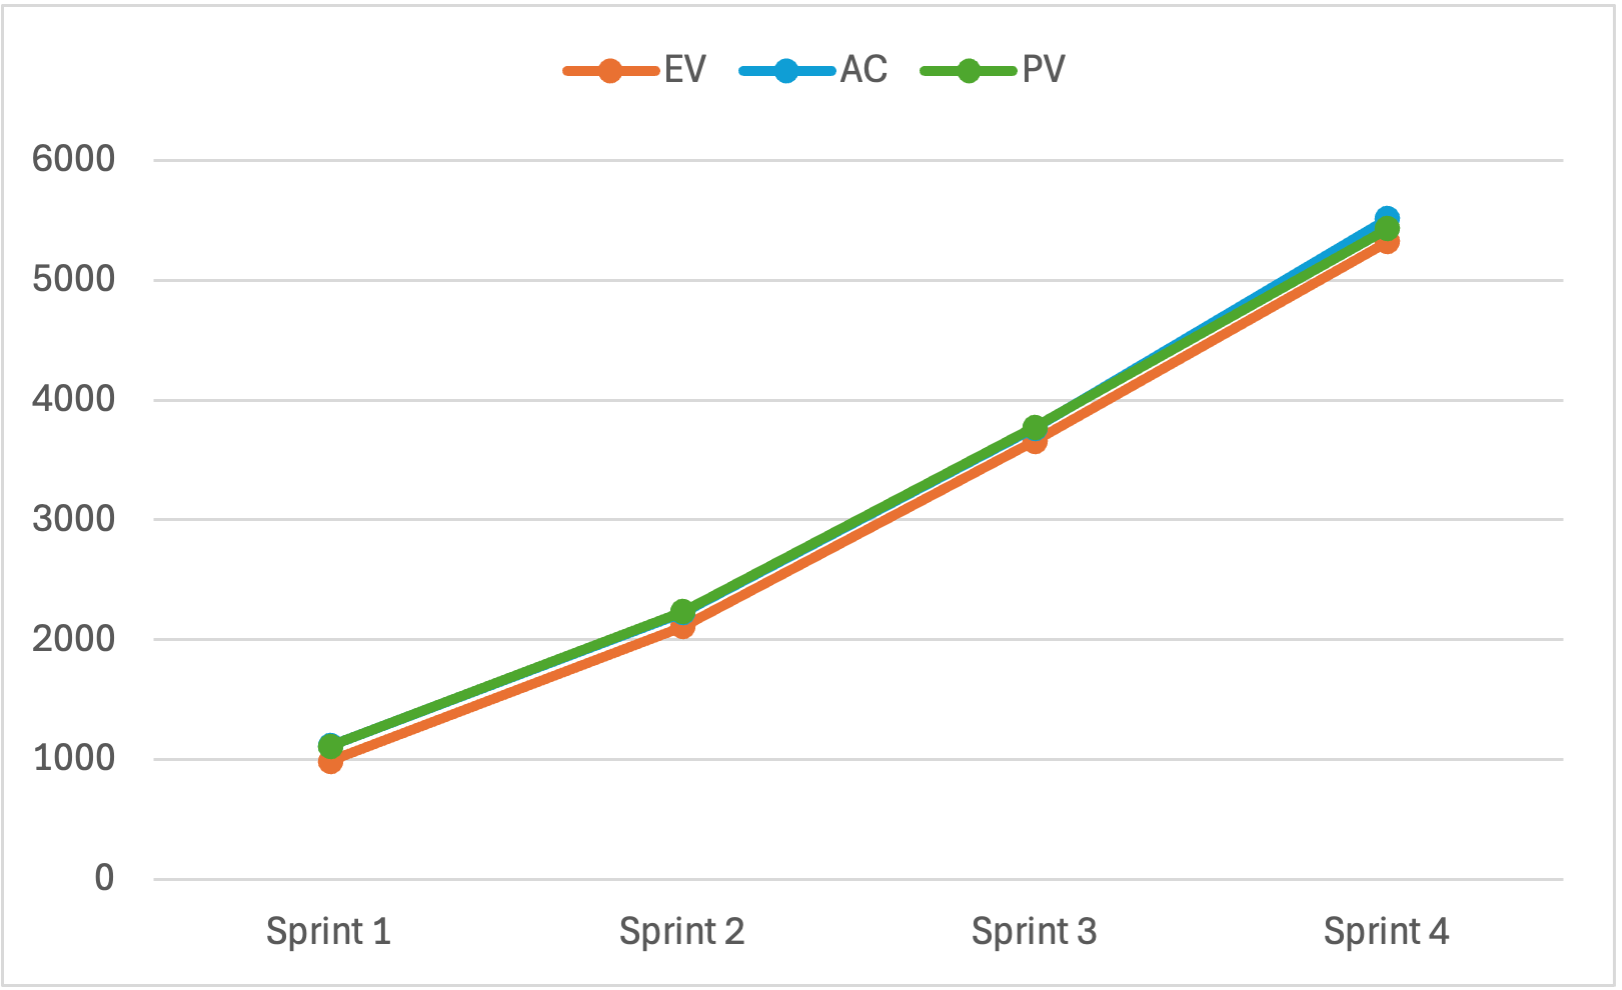
\includegraphics[width=0.8\textwidth]{./images/EV-AC-PV.png}
    \caption{Earned Value, Actual Cost, Planned Value}
\end{figure}
\subsubsubsection*{Analisi}
Queste metriche indicano un buon andamento essendo sempre abbastanza sovrapposte su tutti gli \textit{sprint\textsubscript{G}}, anche se si nota un graduale distaccamento verso il quarto \textit{sprint\textsubscript{G}} a causa dell'aumento dei costi per il raggiungimento degli obiettivi.

\subsubsection{Estimated To Completion, Estimated At Completion}
\begin{figure}[H]
    \centering
    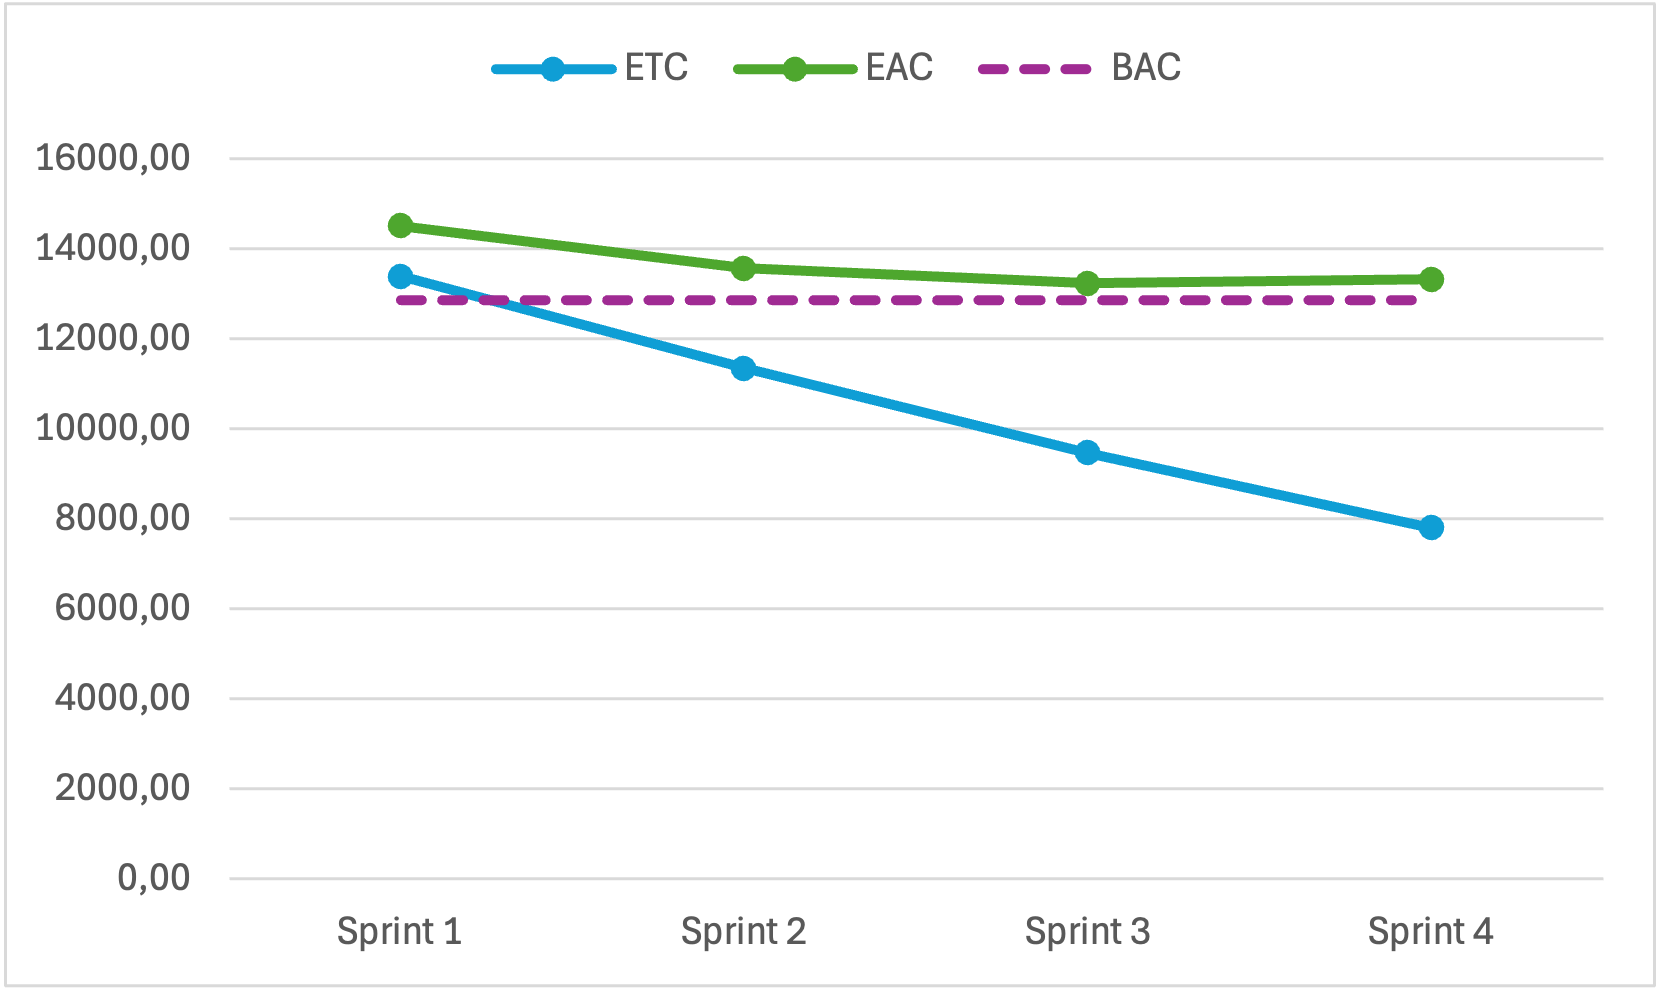
\includegraphics[width=0.8\textwidth]{./images/ETC-EAC.png}
    \caption{Estimated To Completion, Estimated At Completion}
\end{figure}
\subsubsubsection*{Analisi}
Dopo un inizio non ottimale è possibile notare un riallineamento. L'Estimation At Completion si è riallineato al Budget At Completion, ma è sempre rimasto superiore, anche se di poco, a causa del costo maggiore per il raggiungimento di tutti gli obiettivi degli \textit{sprint\textsubscript{G}}. L'Estimated To Completion è sempre stato gradualmente discendente.

\subsubsection{Budget Variance}
\begin{figure}[H]
    \centering
    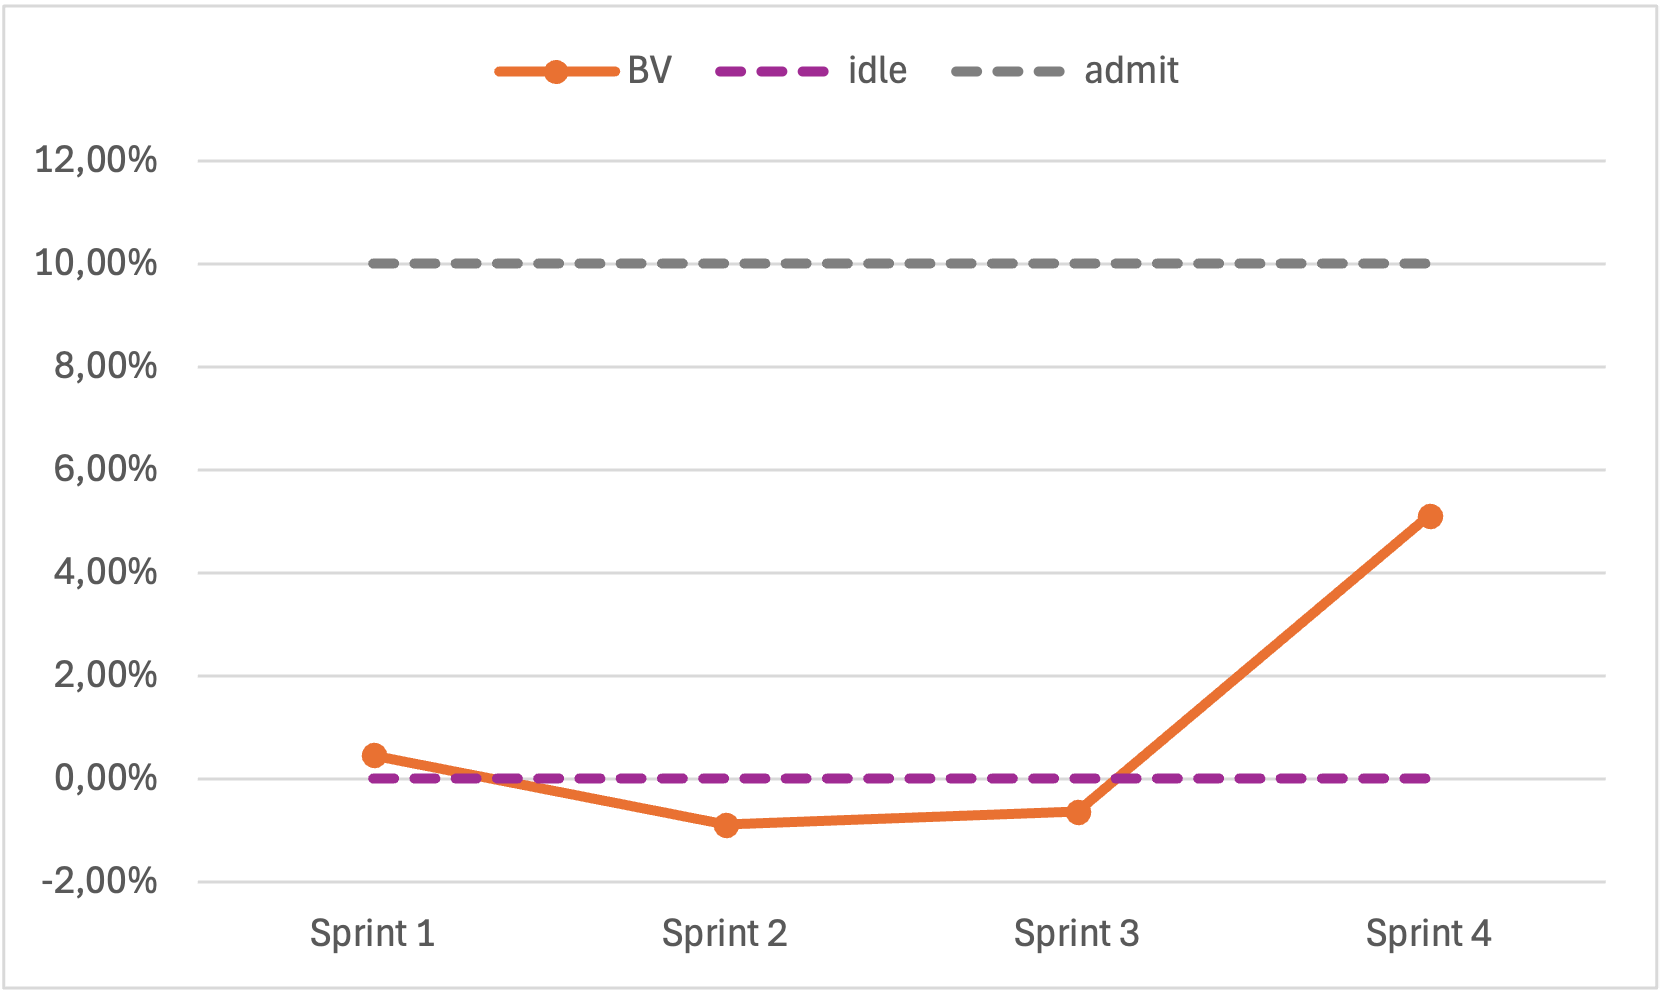
\includegraphics[width=0.8\textwidth]{./images/BV.png}
    \caption{Estimated To Completion, Estimated At Completion}
\end{figure}
\subsubsubsection*{Analisi}
Anche se la Budget Variance è sempre rimasta nei limiti ammissibili, è evidente come nel quarto \textit{sprint\textsubscript{G}}, dove la variazione è notevole, le ore preventivate fossero insufficienti e questo deve spingere a una più corretta pianificazione basata sulle retrospettive precedenti.

\subsubsection{Cost Variance, Schedule Variance}
\begin{figure}[H]
    \centering
    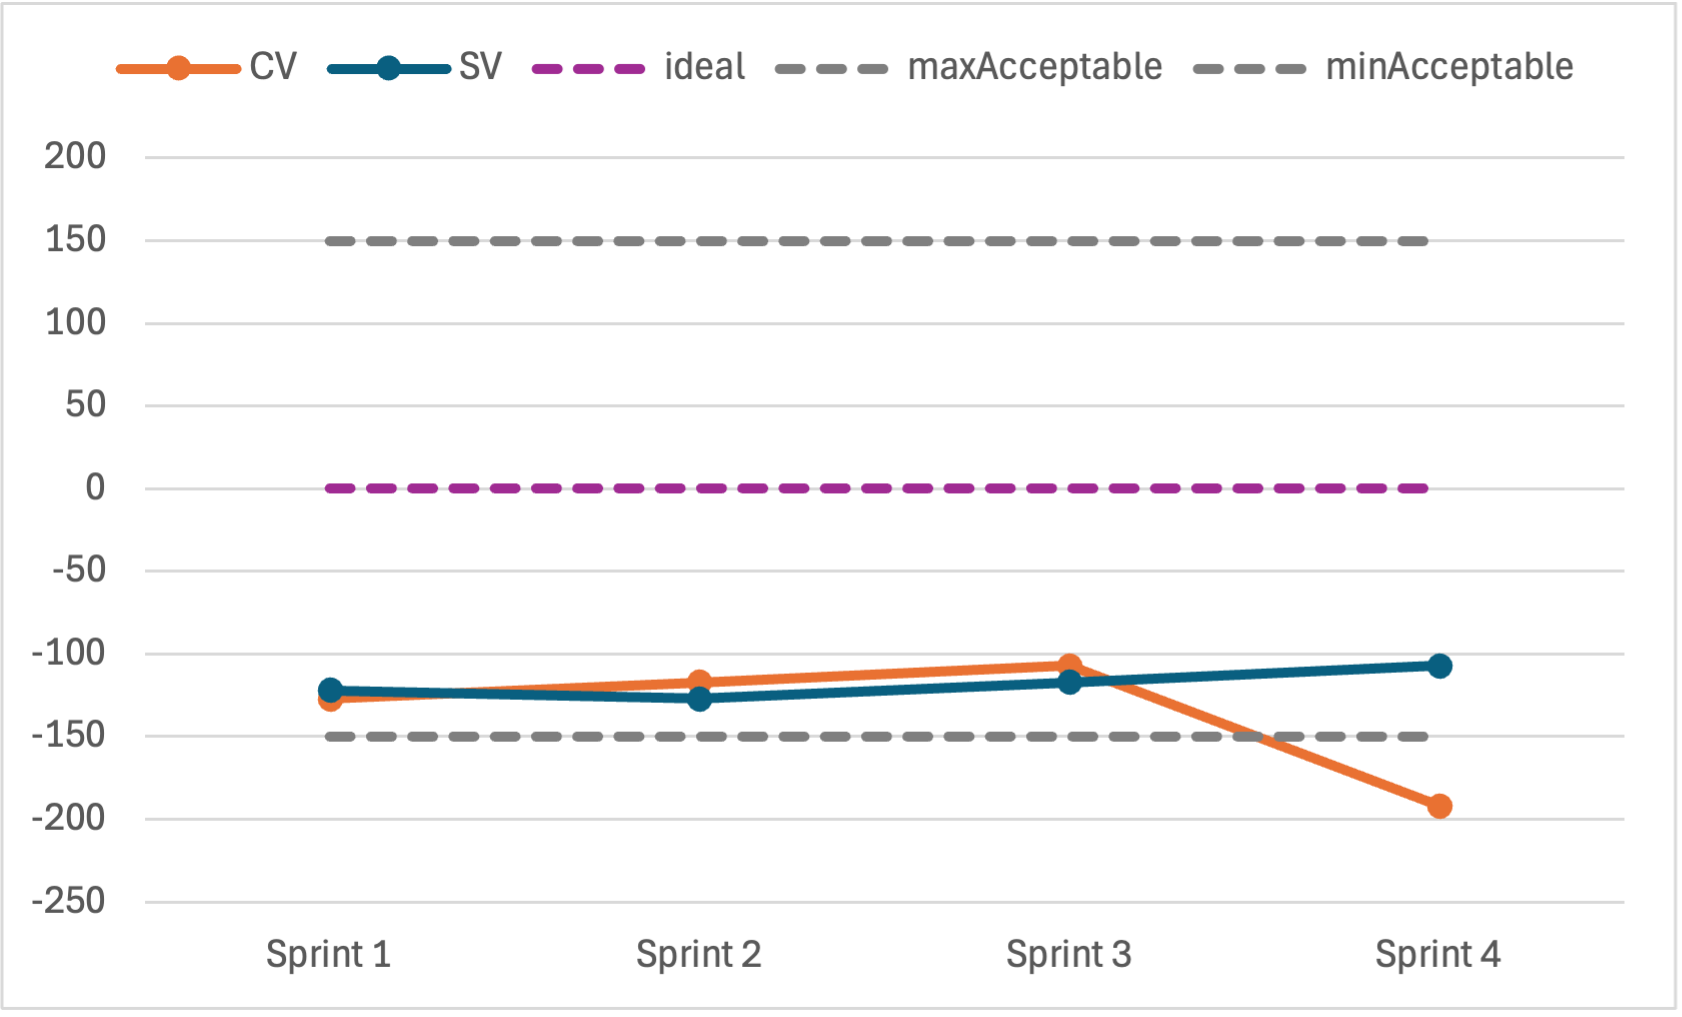
\includegraphics[width=0.8\textwidth]{./images/CV-SV.png}
    \caption{Cost Variance, Schedule Variance}
\end{figure}
\subsubsubsection*{Analisi}
Per quanto i valori, soprattutto della Schedule Variance, siano praticamente sempre rimasti accettabili, non si notano dei netti miglioramenti, ma anzi un peggioramento, come in altre metriche, nel corso del quarto \textit{sprint\textsubscript{G}}. Questo deve spingere a una migliore gestione delle \textit{risorse\textsubscript{G}} per il raggiungimento degli obiettivi entro i costi preventivati.

\subsubsection{Cost Performance Index}
\begin{figure}[H]
    \centering
    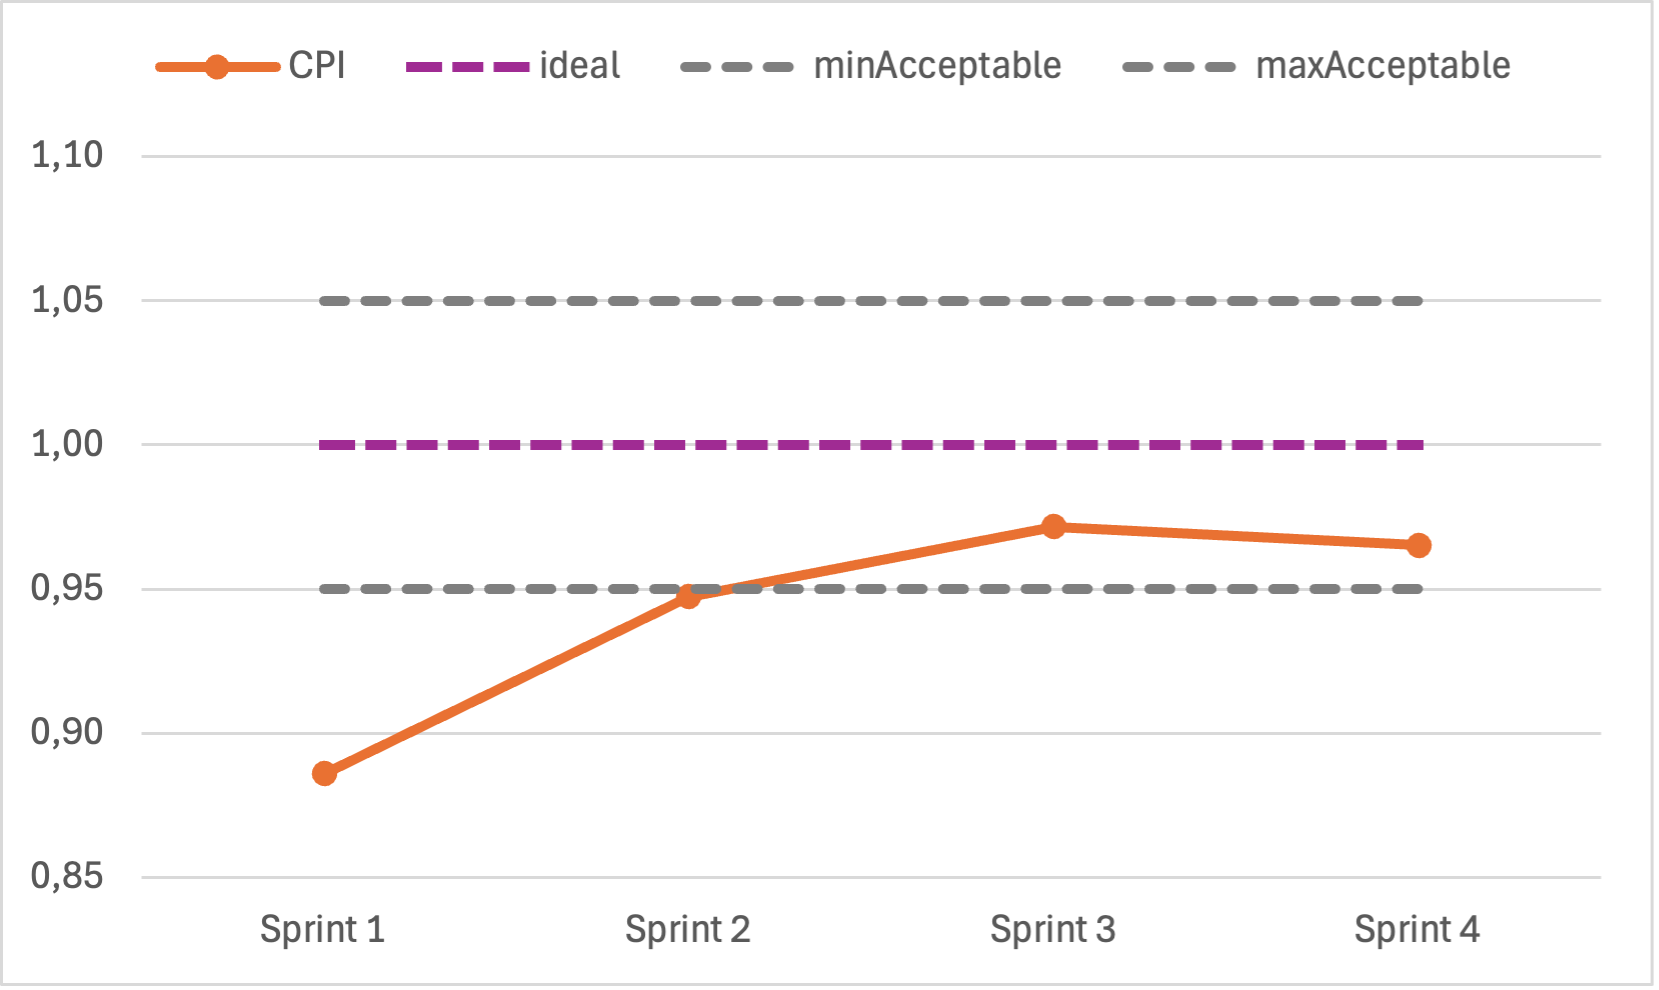
\includegraphics[width=0.8\textwidth]{./images/CPI.png}
    \caption{Cost Performance Index}
\end{figure}
\subsubsubsection*{Analisi}
È evidente come il Cost Performance Index sia migliorato nel corso degli \textit{sprint\textsubscript{G}}, fino a rientrare nei limiti ammissibili, l'obiettivo deve essere quello di seguire il trend attuale per puntare al valore ideale.

\subsection{Qualità di processo - Documentazione}
\subsubsection{Indice di Gulpease}
\begin{figure}[H]
    \centering
    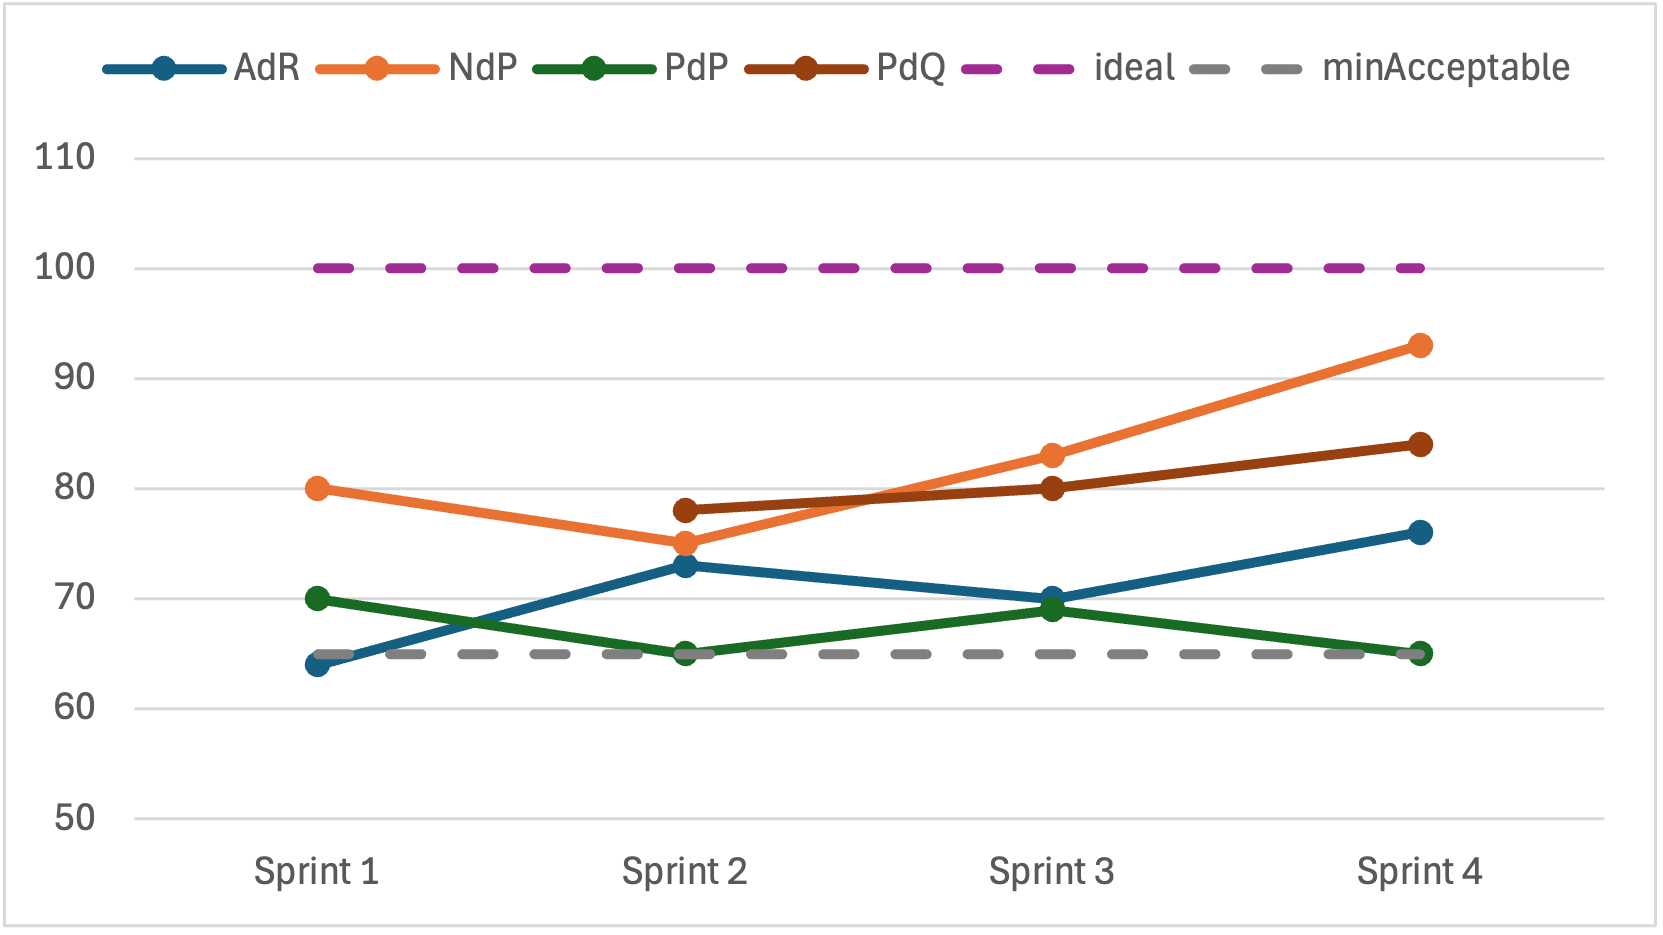
\includegraphics[width=0.8\textwidth]{./images/gulpease.png}
    \caption{Indice di Gulpease}
\end{figure}
\subsubsubsection*{Analisi}
Al termine del secondo \textit{sprint\textsubscript{G}} tutti i documenti erano in lavorazione ed entro i limiti minimi di leggibilità, si nota peraltro un miglioramento nella leggibilità di tutti i documenti ad esclusione del Piano di Progetto, sul quale il gruppo dovrà concentrarsi di più per garantire una scrittura comprensibile.

\subsection{Qualità di processo - Gestione della qualità}
\subsubsection{Metriche non soddisfatte}
\begin{figure}[H]
    \centering
    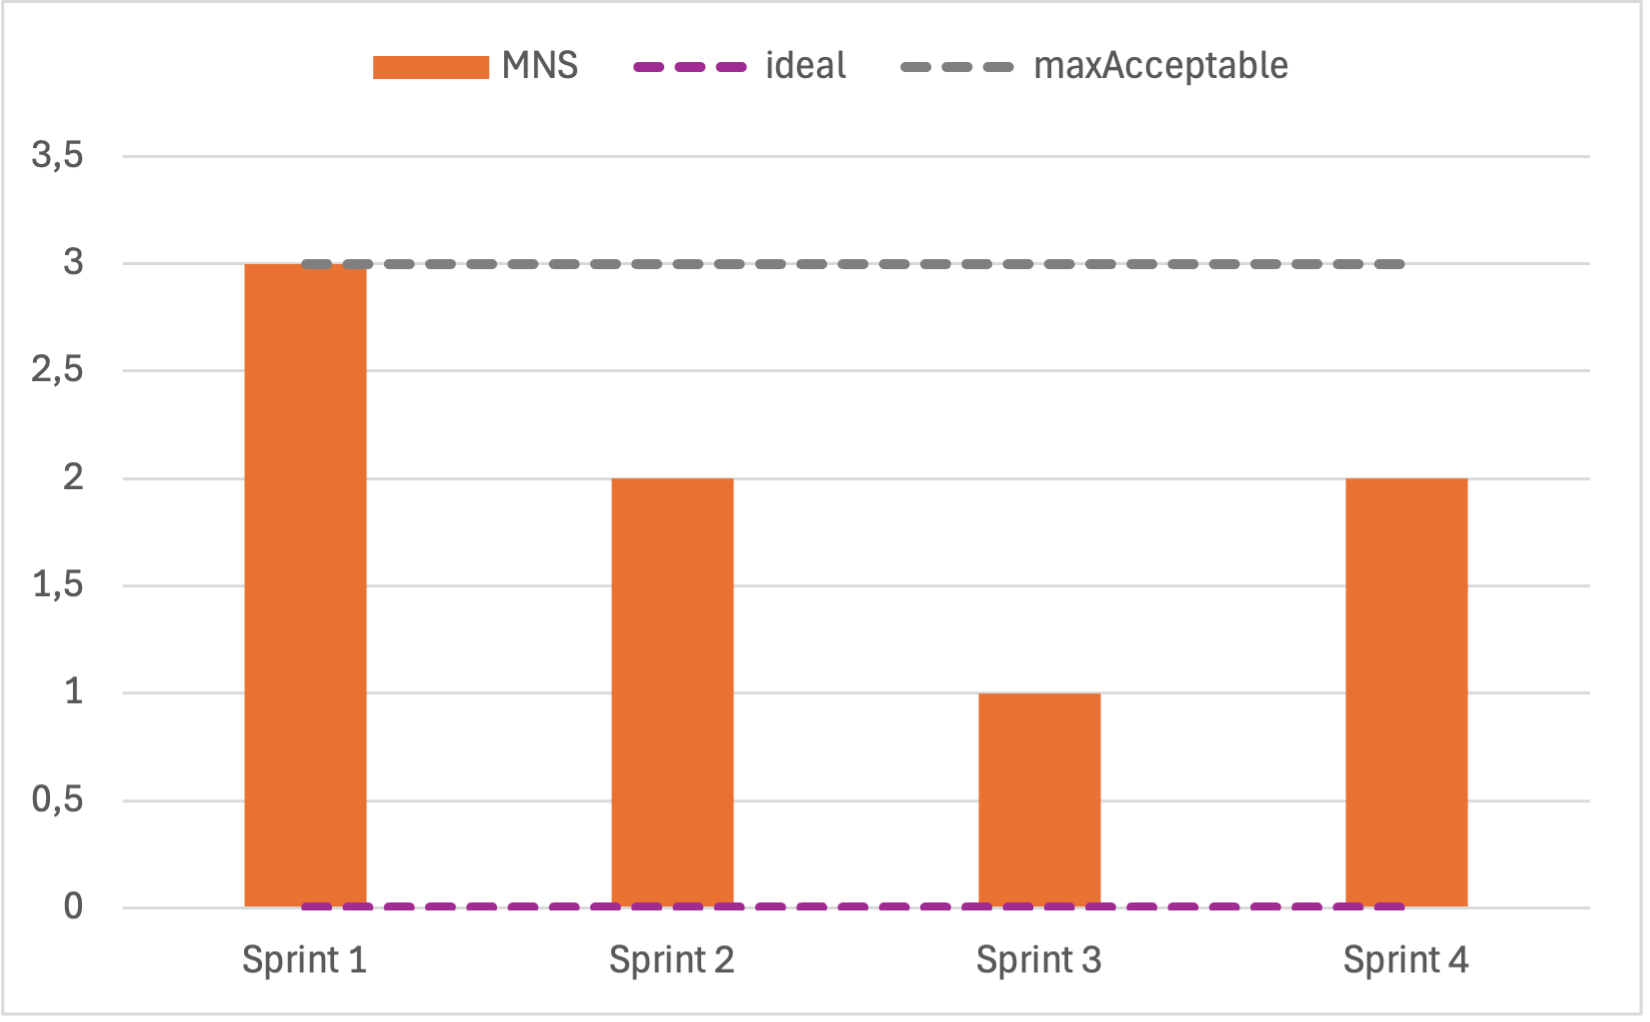
\includegraphics[width=0.8\textwidth]{./images/MNS.png}
    \caption{Metriche non soddisfatte}
\end{figure}
\subsubsubsection*{Analisi}
La metrica che non risulta mai soddisfatta è EAC per la quale si rimanda all'analisi specifica. Altre metriche che risultano non soddisfatte sono ETC (primi due \textit{sprint\textsubscript{G}}), CPI (primo \textit{sprint\textsubscript{G}}) e CV (quarto \textit{sprint\textsubscript{G}} per il quale si rimanda all'analisi specifica).

\subsection{Qualità di prodotto - Funzionalità}
\subsubsection{Requisiti soddisfatti}
\begin{figure}[H]
    \centering
    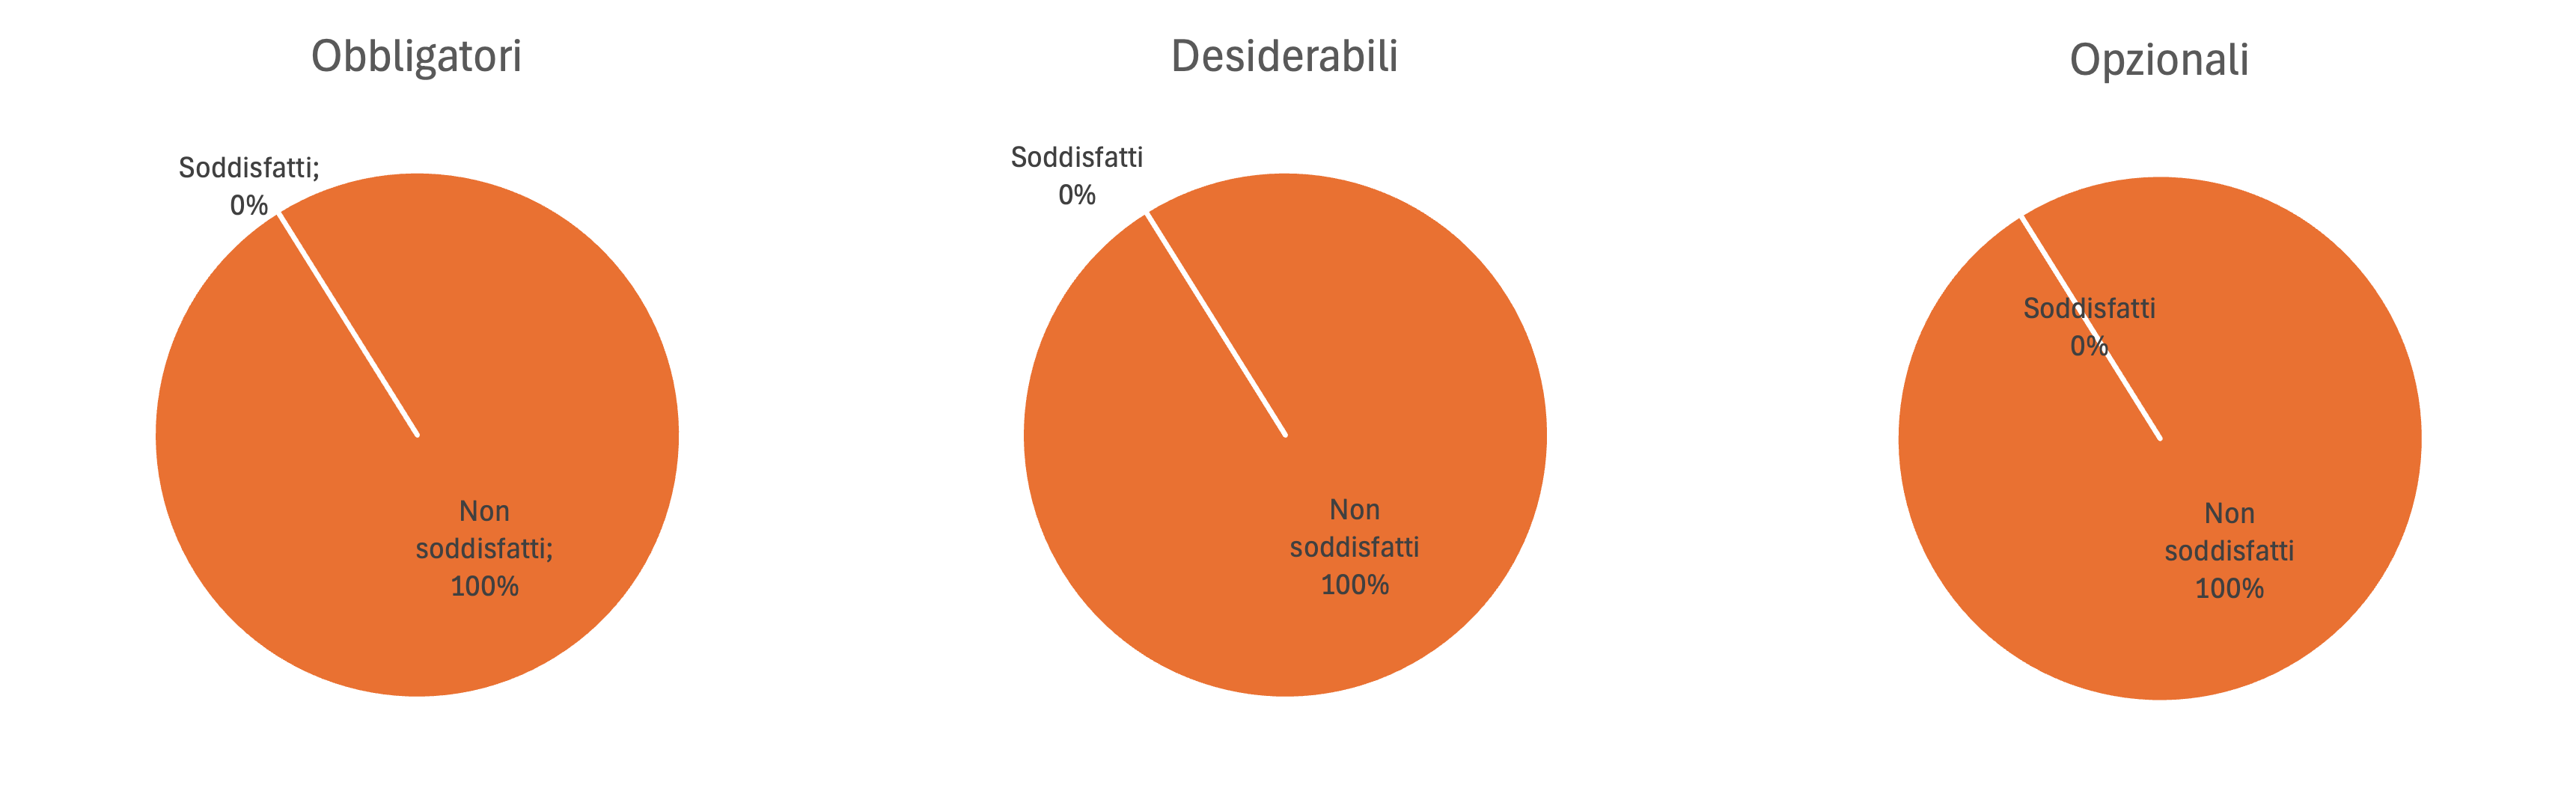
\includegraphics[width=0.8\textwidth]{./images/requisitisoddisfatti.png}
    \caption{Requisiti soddisfatti}
\end{figure}
\subsubsubsection*{Analisi}
Il progetto fino ad ora si è concentrato sulla creazione di un \textit{Proof of Concept\textsubscript{G}}, e non su prodotto finale con il quale soddisfare i \textit{requisiti\textsubscript{G}}, per cui è normale che nel cruscotto non risulti soddisfatto alcun \textit{requisito\textsubscript{G}}.

\subsection{Considerazioni finali in vista della revisione RTB}
Sin dalle prime fasi del progetto il gruppo si è posto l'obiettivo di avere un \textit{Way of Working\textsubscript{G}} chiaro e puntuale, anche se di natura incrementale, in quanto questo deve essere gradualmente ampliato e raffinato con il passare del tempo. Nonostante il \textit{Way of Working\textsubscript{G}} sia progressivamente migliorato con l’avanzare del progetto, alcune aree necessitano di essere ancora migliorate per far sì che la qualità di processo si rifletta positivamente sulla qualità di prodotto. \\
La comunicazione, all'interno del team e con il Proponente\textsubscript{G} è stata fin da subito stabile e costruttiva, sia in modalità sincrona, permettendo riunioni efficaci di durata non eccessiva, che asincrona, permettendo una buona organizzazione del lavoro. \\
Il processo di automiglioramento che il gruppo si è impegnato ad assumere si è concentrato, e continuerà a concentrarsi, anche sulle modalità di gestione delle difficoltà e degli imprevisti, per escogitare contromisure efficaci che permettano di non sprecare \textit{risorse\textsubscript{G}}. \\
Un obiettivo di vitale importanza per il gruppo nel corso dei prossimi \textit{sprint\textsubscript{G}} è l'aggiornamento rigoroso e puntuale del Piano di Progetto e del Piano di Qualifica con i dati rilevanti ed aggiornati, al fine da poter essere sfruttati al meglio. \\
x